%%%%%%%%%%%%%%%%%%%%%%%%%%%%%%%%%%%%%%%%%
% Masters/Doctoral Thesis 
% LaTeX Template
% Version 2.2 (21/11/15)
%
% This template has been downloaded from:
% http://www.LaTeXTemplates.com
%
% Version 2.x major modifications by:
% Vel (vel@latextemplates.com)
%
% This template is based on a template by:
% Steve Gunn (http://users.ecs.soton.ac.uk/srg/softwaretools/document/templates/)
% Sunil Patel (http://www.sunilpatel.co.uk/thesis-template/)
%
% Template license:
% CC BY-NC-SA 3.0 (http://creativecommons.org/licenses/by-nc-sa/3.0/)
%
%%%%%%%%%%%%%%%%%%%%%%%%%%%%%%%%%%%%%%%%%

%----------------------------------------------------------------------------------------
%	PACKAGES AND OTHER DOCUMENT CONFIGURATIONS
%----------------------------------------------------------------------------------------

\documentclass[
11pt, % The default document font size, options: 10pt, 11pt, 12pt
%oneside, % Two side (alternating margins) for binding by default, uncomment to switch to one side
english, % ngerman for German
singlespacing, % Single line spacing, alternatives: onehalfspacing or doublespacing
%draft, % Uncomment to enable draft mode (no pictures, no links, overfull hboxes indicated)
%nolistspacing, % If the document is onehalfspacing or doublespacing, uncomment this to set spacing in lists to single
%liststotoc, % Uncomment to add the list of figures/tables/etc to the table of contents
%toctotoc, % Uncomment to add the main table of contents to the table of contents
%parskip, % Uncomment to add space between paragraphs
%nohyperref, % Uncomment to not load the hyperref package
headsepline, % Uncomment to get a line under the header
]{MastersDoctoralThesis} % The class file specifying the document structure

\usepackage[utf8]{inputenc} % Required for inputting international characters
\usepackage[T1]{fontenc} % Output font encoding for international characters

\usepackage{palatino} % Use the Palatino font by default

\usepackage[backend=bibtex,style=numeric,natbib=true ,bibencoding=ascii]{biblatex} % User the bibtex backend with the authoryear citation style (which resembles APA)

\addbibresource{example.bib} % The filename of the bibliography

\usepackage[autostyle=true]{csquotes} % Required to generate language-dependent quotes in the bibliography

%----------------------------------------------------------------------------------------
%	MARGIN SETTINGS
%----------------------------------------------------------------------------------------

\geometry{
	paper=a4paper, % Change to letterpaper for US letter
	inner=2.5cm, % Inner margin
	outer=3.8cm, % Outer margin
	bindingoffset=2cm, % Binding offset
	top=1.5cm, % Top margin
	bottom=1.5cm, % Bottom margin
	%showframe,% show how the type block is set on the page
}

%----------------------------------------------------------------------------------------
%	THESIS INFORMATION
%----------------------------------------------------------------------------------------

\thesistitle{RSSI \& Magnetometer based fingerprinting localization in indoor wireless environments} % Your thesis title, this is used in the title and abstract, print it elsewhere with \ttitle
%\title{Bachelors Thesis Carl Balmer}
\supervisor{Jose \textsc{Carerra}} % Your supervisor's name, this is used in the title page, print it elsewhere with \supname
\examiner{} % Your examiner's name, this is not currently used anywhere in the template, print it elsewhere with \examname
\degree{Bachelor of Science in Computer Science} % Your degree name, this is used in the title page and abstract, print it elsewhere with \degreename
\author{Carl \textsc{Balmer}} % Your name, this is used in the title page and abstract, print it elsewhere with \authorname
\addresses{Bantigerstrasse 49\\3006 Bern} % Your address, this is not currently used anywhere in the template, print it elsewhere with \addressname

\subject{Indoor Localization} % Your subject area, this is not currently used anywhere in the template, print it elsewhere with \subjectname
\keywords{} % Keywords for your thesis, this is not currently used anywhere in the template, print it elsewhere with \keywordnames
\university{\href{http://www.unibe.ch}{Universität Bern}} % Your university's name and URL, this is used in the title page and abstract, print it elsewhere with \univname
\department{\href{http://www.inf.unibe.ch/}{Institute of Computer Science}} % Your department's name and URL, this is used in the title page and abstract, print it elsewhere with \deptname
\group{\href{http://www.cds.unibe.ch}{Communication and Distributed Systems}} % Your research group's name and URL, this is used in the title page, print it elsewhere with \groupname
\faculty{\href{http://www.philnat.unibe.ch/}{Faculty of Science}} % Your faculty's name and URL, this is used in the title page and abstract, print it elsewhere with \facname

\hypersetup{pdftitle=\ttitle} % Set the PDF's title to your title
\hypersetup{pdfauthor=\authorname} % Set the PDF's author to your name
\hypersetup{pdfkeywords=\keywordnames} % Set the PDF's keywords to your keywords

\begin{document}

\frontmatter % Use roman page numbering style (i, ii, iii, iv...) for the pre-content pages

\pagestyle{plain} % Default to the plain heading style until the thesis style is called for the body content

%----------------------------------------------------------------------------------------
%	TITLE PAGE
%----------------------------------------------------------------------------------------

\begin{titlepage}
\begin{center}

\textsc{\LARGE \univname}\\[1.5cm] % University name
\textsc{\Large Bachelor Thesis}\\[0.5cm] % Thesis type

\HRule \\[0.4cm] % Horizontal line
{\huge \bfseries \ttitle}\\[0.4cm] % Thesis title
\HRule \\[1.5cm] % Horizontal line
 
\begin{minipage}{0.4\textwidth}
\begin{flushleft} \large
\emph{Author:}\\
\authorname % Author name - remove the \href bracket to remove the link
\end{flushleft}
\end{minipage}
\begin{minipage}{0.4\textwidth}
\begin{flushright} \large
\emph{Supervisor:} \\
\supname % Supervisor name - remove the \href bracket to remove the link  
\end{flushright}
\end{minipage}\\[3cm]
 
\large \textit{A thesis submitted in fulfillment of the requirements\\ for the degree of \degreename}\\[0.3cm] % University requirement text
\textit{in the}\\[0.4cm]
\groupname\\\deptname\\[2cm] % Research group name and department name
 
{\large \today}\\[2cm] % Date

\includegraphics[scale=0.4]{Logo} % University/department logo - uncomment to place it
 
\vfill
\end{center}
\end{titlepage}

%----------------------------------------------------------------------------------------
%	DECLARATION PAGE
%----------------------------------------------------------------------------------------

\begin{declaration}
\addchaptertocentry{\authorshipname}

\noindent Ich erkläre hiermit, dass ich diese Arbeit selbstständig verfasst und keine anderen als die angegebenen Quellen benutzt habe. Alle Stellen, die wörtlich oder sinngemäss aus Quellen entnommen wurden, habe ich als solche gekennzeichnet. Mir ist bekannt, dass andernfalls der Senat gemäss Artikel 36 Absatz 1 Buchstabe r des Gesetzes vom 5. September 1996 über die Universität zum Entzug des auf Grund dieser Arbeit verliehenen Titels berechtigt ist.\\[2cm]


\noindent Signed:\\
\rule[0.5em]{25em}{0.5pt} % This prints a line for the signature
 
\noindent Date:\\
\rule[0.5em]{25em}{0.5pt} % This prints a line to write the date
\end{declaration}

\cleardoublepage

%----------------------------------------------------------------------------------------
%	QUOTATION PAGE
%----------------------------------------------------------------------------------------

\vspace*{0.2\textheight}

\noindent\enquote{\itshape One thing I've learned: you can know anything, it's all there, you just have to find it.}\bigbreak

\hfill Neil Gaiman

%----------------------------------------------------------------------------------------
%	ABSTRACT PAGE
%----------------------------------------------------------------------------------------

\begin{abstract}
\addchaptertocentry{\abstractname} % Add the abstract to the table of contents

The Thesis Abstract is written here (and usually kept to just this page). The page is kept centered vertically so can expand into the blank space above the title too\ldots

\end{abstract}

%----------------------------------------------------------------------------------------
%	ACKNOWLEDGEMENTS
%----------------------------------------------------------------------------------------

\begin{acknowledgements}
\addchaptertocentry{\acknowledgementname} % Add the acknowledgements to the table of contents

\noindent I would like to thank in particular Jose Carerra for supervising this thesis and his support on various occasions during my work on this thesis.

Further thanks goes to Viviane Tanner and Martina Föhn for their individual support on this thesis.

\end{acknowledgements}

%----------------------------------------------------------------------------------------
%	LIST OF CONTENTS/FIGURES/TABLES PAGES
%----------------------------------------------------------------------------------------

\tableofcontents % Prints the main table of contents

\listoffigures % Prints the list of figures

\listoftables % Prints the list of tables

%----------------------------------------------------------------------------------------
%	ABBREVIATIONS
%----------------------------------------------------------------------------------------

\begin{abbreviations}{ll} % Include a list of abbreviations (a table of two columns)

\textbf{AN} & \textbf{A}nchor \textbf{N}ode\\
\textbf{MN} & \textbf{M}obile \textbf{N}ode\\
\textbf{CDS} & \textbf{C}ommunication and \textbf{D}istributed \textbf{S}ystems\\
\textbf{RSSI} & \textbf{R}eceived \textbf{S}ignal \textbf{S}trength \textbf{I}ndicator\\
\textbf{OLS} & \textbf{O}rdinary \textbf{L}east \textbf{S}quares\\
\textbf{WLS} & \textbf{W}eighted \textbf{L}east \textbf{S}quares\\

\end{abbreviations}

%----------------------------------------------------------------------------------------
%	PHYSICAL CONSTANTS/OTHER DEFINITIONS
%----------------------------------------------------------------------------------------

\begin{constants}{lr@{${}={}$}l} % The list of physical constants is a three column table

% The \SI{}{} command is provided by the siunitx package, see its documentation for instructions on how to use it

	Speed of Light & $c_{0}$ & \SI{2.99792458e8}{\meter\per\second} (exact)\\
%Constant Name & $Symbol$ & $Constant Value$ with units\\

\end{constants}

%----------------------------------------------------------------------------------------
%	SYMBOLS
%----------------------------------------------------------------------------------------

\begin{symbols}{lll} % Include a list of Symbols (a three column table)

$a$ & distance & \si{\meter} \\
$P$ & power & \si{\watt} (\si{\joule\per\second}) \\
%Symbol & Name & Unit \\

\addlinespace % Gap to separate the Roman symbols from the Greek

$\omega$ & angular frequency & \si{\radian} \\

\end{symbols}

%----------------------------------------------------------------------------------------
%	DEDICATION
%----------------------------------------------------------------------------------------

\dedicatory{Dedicated to a cookie - You are always such a good placeholder\ldots} 

%----------------------------------------------------------------------------------------
%	THESIS CONTENT - CHAPTERS
%----------------------------------------------------------------------------------------

\mainmatter % Begin numeric (1,2,3...) page numbering

\pagestyle{thesis} % Return the page headers back to the "thesis" style

% Include the chapters of the thesis as separate files from the Chapters folder
% Uncomment the lines as you write the chapters

% Chapter 1

\chapter{Introduction} % Main chapter title

\label{Chapter1} % For referencing the chapter elsewhere, use \ref{Chapter1} 

%----------------------------------------------------------------------------------------

% Define some commands to keep the formatting separated from the content 
\newcommand{\keyword}[1]{\textbf{#1}}
\newcommand{\tabhead}[1]{\textbf{#1}}
\newcommand{\code}[1]{\texttt{#1}}
\newcommand{\file}[1]{\texttt{\bfseries#1}}
\newcommand{\option}[1]{\texttt{\itshape#1}}

%----------------------------------------------------------------------------------------

The main focus of this thesis is indoor localization of mobile devices especially smartphones.

With today's ubiquity of mobile computing, it has become evermore important for these devices to be aware of their location. Location awareness is fundamental for many possible applications such as pedestrian navigation and location based marketing in large building complexes (e.g. universities, airports, hospitals) or audio-guides for museums.

In contrast to outdoor localization, where we have GPS and other established solutions, indoor localization still remains challenging. Some of the reasons for this include the inability of the GPS signal to penetrate into the building and the effects of non-line-of-sight and multipath propagation on radio waves deteriorating the signal to be less accurate for localization\cite{JoseMaster,multipathEffects}. In addition to these challenges indoor location based applications usually require higher accuracy than those outdoors; An error of four meters is acceptable for street navigation but not for a museum guide.

\section{Motivation}

This has been an active research field in the last few years with many different techniques proposed \cite{surveyIndoorTechniques,surveyWirelessPersonal}. One common approach is to base the localization on WiFi radio signals. WiFi infrastructure is already present in almost every building and can easily be upgraded with standardized off the shelf hardware. These radio-based techniques are usually classified into range-based and range-free methods\cite{FineGrainedIndoorTracking}.

Fingerprinting is a common range-free method, where known radio parameters are mapped to a location. Later this map is used to determine the devices location based on the current radio parameters. Fingerprinting can achieve good accuracy but creating the map is very labor intensive\cite{FineGrainedIndoorTracking}.

Range-based methods use the radio parameters to try to approximate the distance between the mobile device (Mobile Node) and the signal emitters (Anchor Nodes). This process is called ranging. Trilateration is then performed on these distances to determine the position of the MN. The ranging process is prone to errors caused by multipath propagation.\cite{FineGrainedIndoorTracking}.

%----------------------------------------------------------------------------------------
\section{Overview and Contributions}

Previous research at the CDS group used the smartphones received signal strength indicator in a range-based approach, using a regression model for ranging and least squares optimization for solving the trilateration problem \note{Citation needed}.In this work I investigate if this approach can be improved by adding a room recognition layer to it. I use the room recognition to assign weights to the ranges based on the devices current room and so improve the trilateration with weighted least squares. For the room recognition I employ a fingerprinting map built from the RSSI and the magnetic field readings of the smartphones internal magnetometer.\\

My main findings are summarized as follows:
\begin{itemize}
\item The proposed room recognition method is feasible, has sufficiently high accuracy and the map is not very labor intensive to create \note{Formulation}.
\item The inclusion of magnetic field data significantly improves the accuracy of the room recognition.
\item Setting weights based on the room recognition increases the trilaterations accuracy, although not very significantly.
\end{itemize}

\section{Structure of this Work}

\noindent In the remainder of this work, \red{related works} and the theoretical background is reviewed in chapter 2. The room recognition approach is introduced and investigated in chapter 3, the weighting methods in chapter 4. In chapter 5 the methods from the previous chapters are then evaluated. Chapter 6 concludes the thesis. \\\note{Rewrite this part}\\\note{rework the section headings and page beak}
% Chapter Template

\chapter{Theoretical Background} % Main chapter title

\label{Chapter2} % Change X to a consecutive number; for referencing this chapter elsewhere, use \ref{ChapterX}

Indoor localization has been a active research field in the last few years. In this chapter the two most common approaches, fingerprinting and range-based, are introduced and their components explained in detail. For the fingerprinting approach I will also talk about \emph{support vector machines} and \emph{the magnetic field in indoor environments}. Although they are not normally used in with fingerprinting they play a vital role in the room recognition system proposed in chapter \ref{Chapter3}. So understanding these concepts will be important.

\section{Range-Based Localization}
\label{therory:range-based}

A range based localization system consists of two main components.

\textbf{A number of Anchor Nodes (ANs)} which are placed at known locations and constantly transmit a radio signal.

\textbf{A mobile node (MN)}, in this case a smartphone, whose location is unknown and needs to be determined.

\begin{figure}[ht]
\centering
\includegraphics[width=\textwidth]{Figures/existingAproach}
\decoRule
\caption[Range-based localization approach]{Block diagram of the range based localization approach.}
\label{fig:existingApproach}
\end{figure}

To determine its position the mobile node measures the received signal strength from each of the anchor nodes $(RSSI_i)$. A ranging model is then used to estimate the distance $(d_i)$ from the mobile node to each anchor node. Because the location of the anchor nodes is known, it is then possible to calculate the position of the mobile node using trilateration. To account for errors during the ranging step the trilateration can also be provided with a set of weights $(w_i)$ representing the accuracy of each distance estimation.

The range-based approach to localization has the benefit of only requiring  a few training samples to train the ranging models. It is therefore easy and not very labour intensive to implement. The problem is that in indoor environments the ranging models are often inaccurate, limiting the localization accuracy that can be achieved with this approach.

In the following subsections the ranging, trilateration and weighting steps are described in further detail.

\subsection{RSSI and signal propagation}

The received signal strength indicator describes the total signal power received in milliwatts with the value expressed on a logarithmic scale (dBm)\cite[p.~160]{sauter2010gsm}. In the case of Wi-Fi a value of -30 would mean a very strong signal while one of -90 would be so low as to be unusable (drowning in noise). In an open space without any obstacles the RSSI mainly depends on the propagation distance, but indoors several other factors become important. These are non line of sight (NLOS) and multipath propagation.

NLOS occurs when the signals path is obstructed by physical objects. The signal has to pass through these objects and therefore the RSSI is lower compared to LOS, where there are no obstacles\cite{JoseMaster}.

Multypath propagation is caused when the signal is reflected from physical objects and arrives at the receiver multiple times with different signal strength. This causes inaccuracy and fluctuations in the measured RSSI as all these signals are blended together\cite{multipathEffects}.

Both of these affects are very common in indoor environments, caused by the walls, people, furniture and other building materials. Furthermore the RSSI values are discrete and not fine grained what causes additional inaccuracy. This makes range-based localization based on RSSI challenging and limits its accuracy.

There are other ways to assess the signal strength, such as channel state information, which is more fine grained and can mitigate multipath effects, but they are not available on most mobile devices\cite{JoseMaster,FineGrainedIndoorTracking}.

\subsection{Ranging}
\label{Ranging}

The ranging process estimates the distance between the ANs and the MN based on the radio parameters, in this case RSSI. This is done with non-linear regression (NLR) and the following model proposed by \cite{li2015passiveWIFIsource}:
\begin{equation} \label{eqn:non-linear path loss model}
d_{i}=\alpha_{i}e^{\beta_{i}RSSI_{i}}
\end{equation}
It describes the loss of signal strength over the propagation distance. \(d_{i}\) is the estimated distance from the MN to the \(i\)-th AN, \(RSSI_{i}\) is the \(i\)-th AN's signal strength as measured by the MN and \(\alpha_{i}, \beta_{i}\) are environment variables specific to each AN.

The model needs to be trained for each AN individually by determining the values for \(\alpha_{i}\) and \(\beta_{i}\). This is done by fitting the function to a small set of training samples. This can be done using, for example, least squares optimization.

\subsection{Trilateration}

Trilateration is the process of determining a absolute or relative location based on the distance to known locations. In contrast to triangulation it relies on distances instead of angles.

In the context of localization the goal is to determine the NM's location \(\left ( x,y \right )\) based on the the locations of the ANs \(\left ( \tilde{x_{i}},\tilde{y_{i}} \right )\) and the distance estimations \(d_{i}\) obtained from the path loss model.

The actual distance \(D_{i}\) from the MN to the \(i\)-th AN can be expressed as follows:
\begin{equation}
D_{i} = \sqrt{\left ( \tilde{x_{i}}-x \right )^{2}+\left ( \tilde{y_{i}}-y \right )^{2}}
\label{eqn: distance MN to AN_{i}}
\end{equation}
Under the assumption that \(d_{i}=D_{i}\)  this leads to the following equation system:
\begin{equation}
\begin{pmatrix}
d_{1}\\ 
d_{2}\\
\vdots\\
d_{n}
\end{pmatrix}
=
\begin{pmatrix}
\sqrt{\left ( \tilde{x_{1}}-x \right )^{2}+\left ( \tilde{y_{1}}-y \right )^{2}}\\
\sqrt{\left ( \tilde{x_{2}}-x \right )^{2}+\left ( \tilde{y_{2}}-y \right )^{2}} \\
\vdots\\
\sqrt{\left ( \tilde{x_{n}}-x \right )^{2}+\left ( \tilde{y_{n}}-y \right )^{2}}
\end{pmatrix}
\label{eqn: trilateration problem as equation system}
\end{equation}

But \(d_{i}\) is only an estimation so there is no exact solution of the above system. The best solution is the one that minimizes the sum of the squared error \(d_{i} - D_{i}\). So to determine the MN's location the following problem has to be solved:
\begin{equation}
argmin_{x,y}\sum_{i=1}^{n}w_{i}\left ( d_{i} - \sqrt{\left ( \tilde{x_{i}}-x \right )^{2}+\left ( \tilde{y_{i}}-y \right )^{2}} \right )^{2}
\label{eqn: trilateration as optimization problem}
\end{equation}
This can be done using a optimization algorithm like "Levenberg–Marquardt" or "Gauss-Newton".

\subsection{Weighting}

The optimization problem in equation \ref{eqn: trilateration as optimization problem} also defines a set of weights $w_i$ coresponding to each distance estimation $d_i$. In the context of trilateration these weights represent how accurate each distance estimation is.

The ranging models accuracy can vary greatly. By applying a large weight to the more accurate estimations and a small weight to the inaccurate ones it should, in theory, be possible to correct for the ranging error and improve the localization.

In practice the problem is, that the ranging error is not known. A weighting method is needed that estimates the ranging error.

Previous work at the CDS group \cite{FineGrainedIndoorTracking} used the assumption that the ranging error is larger with increasing distance to the anchor node. So the weights were defined as inversely proportional to the estimated distances:

\begin{equation}
w_{i}=\frac{{d_i}^{-1}}{\sum_{n=1}^{N}{d_n}^{-1}}
\label{eqn: distance weights}
\end{equation}

\section{Fingerprinting}

Fingerprinting is a common method for localization based on RSSI\cite{chapre2013RSSI}. It consists of two main phases.

In the offline/training phase a map of reference points (RP) is created by collecting RSSI values for each AN from known locations.
Then in the online phase RSSI values are collected from an unknown location, called the test point (TP). The location of the TP is determined based on the RP-map using machine learning algorithms like  a k-nearest neighbor regression\cite{JoseMaster}.

The accuracy of this method mainly depends on the density of the RP-map. The higher the density of RPs the better the accuracy. Generally achieving a satisfying level of accuracy, requires a lot of RPs. Other factors are the number of attributes in each RP and the variability of the observation parameters.

More attributes per RP, an attribute being a data value like a RSSI or a magnetic field measurement, gives the algorithm more information to work with and so increased the accuracy\cite{Li2012feasableMagnetic}. This effect is subject to diminishing returns\cite{brouwers2014incremental}. A high variability in the observation parameters depending on location is also beneficial.

This approach is able to achieve good accuracies in an indoor environment. The problem is that it is very labour intensive to create the necessary fingerprinting maps.

\subsection{Magnetic field in indoor environments}

Earths natural magnetic field has already been used for localization, mainly as a compass to determine the devices heading in PDR systems. However, the presence of magnetic field anomalies make accurate heading determination difficult for indoor applications. The anomalies are caused by the ferrous structures in the building materials, electrical devices, cables and tubes. Previous research suggests that these anomalies can be used in a fingerprinting approach to determine a devices location\cite{haverinen2009global,angermann2012CharacterizationMagnetic,Li2012feasableMagnetic}. They show that the magnetic field anomalies have sufficient local variability and are mostly stable over time. Therefore they should be applicable for use in localization.

\subsection{Support Vector Machine}
The Support Vector Machine (SVM) is one of the most widely used machine learning algorithms. It predicts the labels of new (unknown) samples based on previous (known) examples. In its basic form it only supports two labels. This is called binary classification.

The known examples are called training data. It consists of instance-label pairs \(\left ( x_{i}, y_{i} \right ), i=1,...,l\) where \(x_{i}\in R^{n}\) and \(y_{i}\in \left \{ -1,1 \right \}\). \(x_{i}\) represents the samples's observable features while the label \(y_{i}\) defines in which category it belongs.

The SVM maps the samples into \(n\)-dimentional space and then tries to fit a hyperplane through that space separating the two classes so that ideally all samples with \(y_{i}=1\) are on one side of the hyperplane and \(y_{i}=-1\) on the other. To make the separation as clear as possible the margin between the hyperplane and the samples is maximized at the same time. The samples which lie directly on the margins are called the support vectors.

To classify a new unknown sample the SVM determines on which side of the hyperplane it lies and assigns the according label.

To fit the hyperpalane the SVM solves the following optimization problem\cite{chang2011libsvm}:
\begin{equation}
\begin{split}
\min_{\omega , b ,\xi}\;\; & \frac{1}{2}\omega^{T}\omega +C\sum_{i=1}^{l}\xi_{i}\\
\textup{subject to}\;\; & y_{i}\left ( \omega^{T}\phi \left ( x_{i} \right )+b \right )\geq 1-\xi_{i},\\
& \xi_{i}\geq 0,i=1,...,l
\end{split}
\end{equation}

There may be outlines in the data, so a hyperplane that separates all samples correctly may not be the best classifier. To account for this, a cost is paid if a sample violates the error term \(y_{i}\left ( w^{T}\phi \left ( x_{i} \right )+b \right )\geq 1\), increasing the objective function by \(C \xi_{i}\). The $C$ parameter defines the trade-off between the simplicity of the decision surface (\emph{hyperplane}) and misclassification of training samples. For large values of $C$ the optimization will chose a hyperplane with a smaller margin, more support vectors and therefore more complex decision surface, trying to classify all samples correctly. Conversely, a small value of $C$ will cause the optimizer to look for a larger-margin separating hyperplane, even if that hyperplane misclassifies some samples\cite{crossValidatedSVMC}.

\begin{figure}[htp]

\label{fig:SVM}
\centering
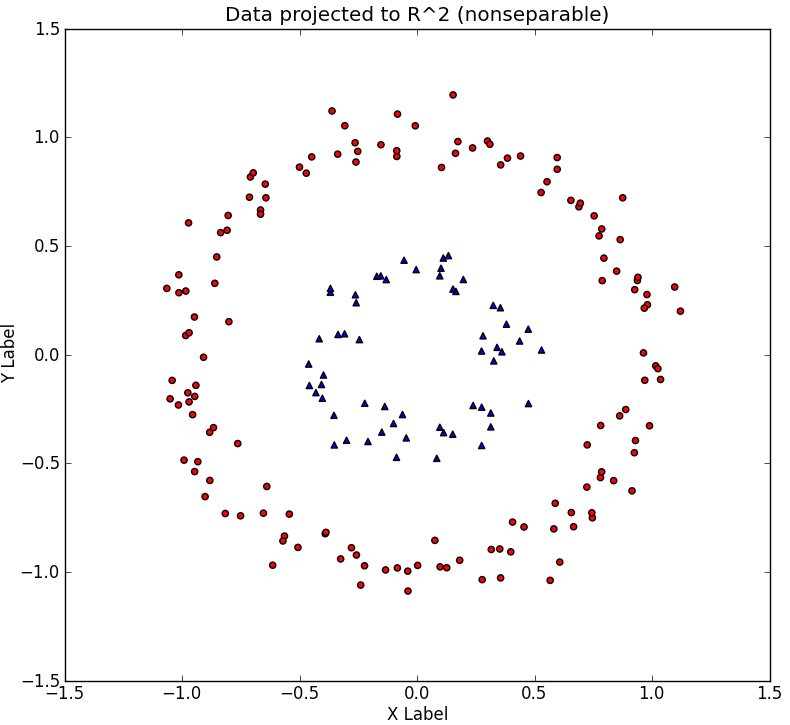
\includegraphics[width=.3\textwidth]{Figures/svm_1.png}\hfill
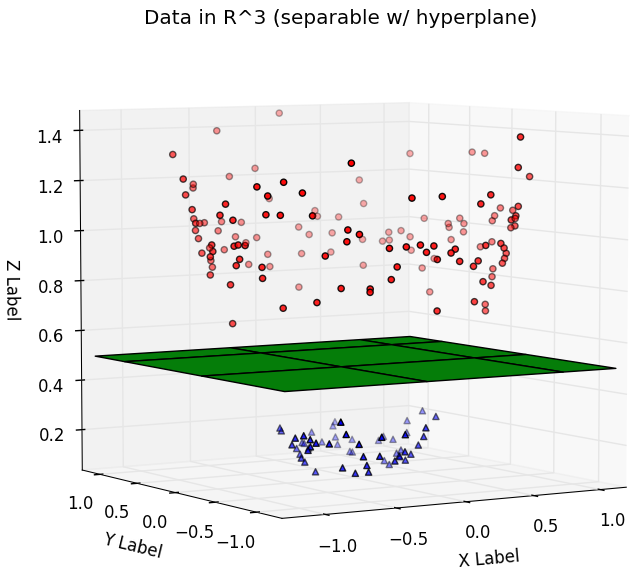
\includegraphics[width=.3\textwidth]{Figures/svm_2.png}\hfill
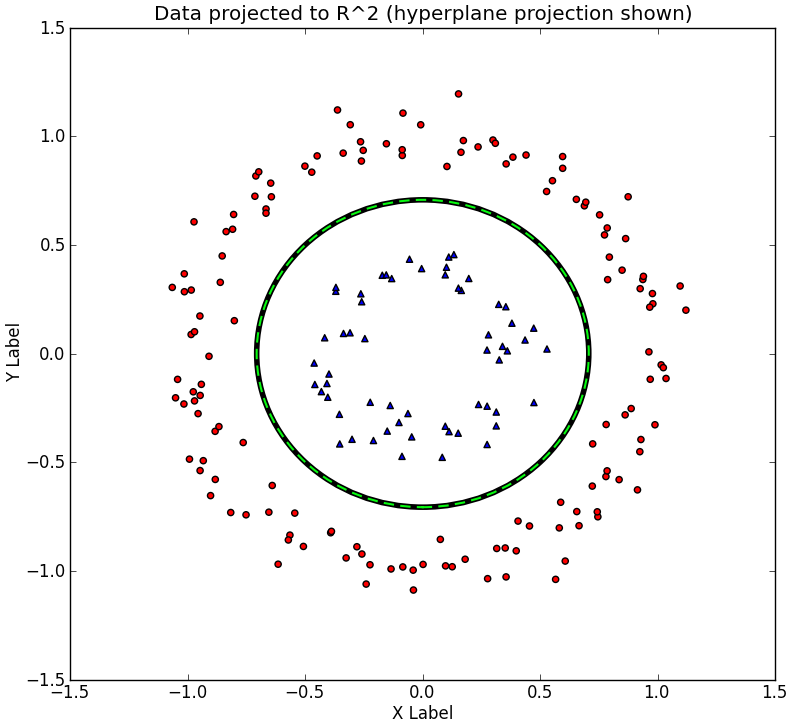
\includegraphics[width=.3\textwidth]{Figures/svm_3.png}
\decoRule
\caption[SVM kernel trick]{\raggedright(Left) A dataset in, not linearly separable. (Middle)The same dataset transformed with decision boundary. (Right) The nonlinear decision boundary.}

\end{figure}

But the training data may not be linearly separable. In this case the so called kernel trick can be used. The kernel is a function \(k\left ( x_{i}, x_{j} \right )=\phi \left ( x_{i} \right )\cdot \phi\left ( x_{j} \right )\) which maps the features \(x_{i}\) to a higher dimensional space where they can be separated by a hyperplane. This results in a non linear separation in the original feature space\cite{ErikKimKernelTrick}.

To perform multy-class classification the "one-against-one" approach can be used. For \(k\) classes \(k\left ( k-1 \right )/2\) classifiers are trained. Each binary classifier is then considered to vote for a class. The sample is then placed in the class with the most votes\cite{chang2011libsvm}.




%----------------------------------------------------------------------------------------
%	OLD
%----------------------------------------------------------------------------------------

 
%\chapter{The localization approach} % Main chapter title

\label{Chapter3} % Change X to a consecutive number; for referencing this chapter elsewhere, use \ref{ChapterX}

In this chapter I will briefly explain the existing localization approach and then go into detail about my proposed improvements.

\section{The existing approach}

The following diagram shows the exiting approach that was used for previous work in the CDS group \cite{josePaper}:

\note{insert diagramm}

It is a range-based approach and consists of two main phases. In the first phase, the training phase, a small number of training samples are gathered from the building. These samples are value-label pairs with the value being the \(RSSIs\) received from the different ANs and the label the \(x,y\) coordinates of the current location in the building. The samples are gathered with a smartphone. \red{In the case of \cite{josePaper} 20 points were used for a floor with approximate 250m\textsuperscript{2} and eight rooms}. The training samples are then used to train the ranging models explained in chapter \ref{Ranging}.

\red{During localization, the second phase,} RSSI readings are provided by the smartphone (MN). These are subsequently converted into distance estimations \(d_i\)  using the ranging models. Trilateration is then applied to determine the smartphones location. The trilateration is ether performed as OLS without any weights or with weights inversely proportional to the estimated distances.

\section{Proposed Improvements}

There is room for improvement in the way that the existing approach determines the trilateration weights. These weights are used to correct for the error introduced by the ranging. So to determine the weights \red{we} need to know the ranging error. The existing approach makes the simple assumption, that the ranging error increases with distance to the AN. \red{This means the error of \(d_i\) is } Supposed that the error is mainly affected by obstructions to the signal (walls, wires etc.). That would mean, that inside one room (where there are no obstructions to the signal) the error should be approximately the same. So if we knew the roon the device is currently in it would be possible to aproxymate the error and determine the weights.

The trilateration weights are used to correct for the error introduced by the ranging

There is room for improvement in the way that the existing approach determines the trilateration weights. These weights represent the accuracy of the distance estimations and it


The existing approach determines the trilateration weights in a very simple method. These weights represent the accuracy of the distance estimation and 
There is room for improvement in the way that the existing 


To determine the weights the existing approach 

assumes that the ranging error increases with distance to the AN. But the ranging error is a function of the location. So I propose to determine the weights using a rougth aproximation of the MN loacation.
I suspect that the ranging error is primarily influenced by obstructions to the Wi-Fi signal (walls, wires etc) and therefore it should be 
It asses the accuracy of \(d_i\) based only on \(d_i\) itself.
The ranging error is a function of the location and I suspect that its main influence are the obstructions to the Wi-Fi signal (walls, wires, etc.) This means that inside a given room the error sould be  
 \red{It is assumed that the ranging error increases with distance to the AN.}
The existing approach asses the accuracy of \(d_i\) based only on \(d_i\) itself. I suspect that the 
\red{I think that the localization can be improved by finding a better way to determine the weights used for the trilateration.} These weights reflect how accurate the estimated distance to a AN is. The existing approach asses the accuracy of \(d_i\) based only on \(d_i\) itself. I propose to assess the accuracy based on the room the device is currently in. This means adding a room recognition layer to the system. Which would detect in which room the device is currently in and, using that knowledge, calculate a set of weights for the trilateration.

\noindent The new approach would look like this:

\note{Insert diagramm here}



This approach requires a simple but reliable method for room room recognition and also a model

that this accuracy is dependent on the location on the device, as the walls between the ANs and the MN change with location. I assume that the accuracy of the estimation is somewhat static inside one room (beacuse there are no majour distuption to the signal). This means that when we already know the room the device in located in, we can can then determine a good set of weights for the trilateration.
So the proposed system would look like this:

\note{insert diagramm}

So the main approach is not changed. There is only a separate room recognition layer that determines the weights \(w_{i}\) for the triangulation.

For this approach to work I need a simple, low cost, method for room recognition and a method to determine the weights based on the knowledge of the room.

\subsection{Room Recognition}
Because the roon recognition layer is only a small part of the location system, ist is not feasible for it to be a complex system, which is very difficult and time consuming to set up and implement. So the goal was to create a room recognition system which required no additional hardware (so it can run in the same environments as the basic approach), uses simple well known technology, and most importantly in not time consuming to implement.

Because of their simplicity I decided to use a fingerprinting approach. The main problem with fingerprinting are the labor intensive maps. But in this case we do not need to measure the exact \((x,y)\)-coordinates of each sample, we only need to label each sample with a room number. This means the map becomes very easy to create, assuming the device has a hight enough samlping rate, one only needs to slowly walk through each room and "scan" it with the smartphone. This can potentially be done in a very short time. 

The second thing to consider are which observation parameters to use as features in the fingerprintng map. In a best case we want a high number of atributes with hight local variability. We use the RSSI values as those are already used for the ranging and trilateration. Aditionally I use the magnetometer readings as previous research has shown its applicably for fingerprinting-localization.

\subsection{Weighting}

During the weighting step of my appoach the set of weights \(w_i\) need to be determined. The information avaliable are the distance estimations \(d_i\) and the output from the room recogniton, the room number. There are a number of different possible ways to do this:

\begin{itemize}
\item inversly proportional to the variance of mesurement errors (in this case distance estimation accuracy)
\item based on the residuals
\item based on the distance
\item calculating optimal weights bevorehand based on known location
\end{itemize}

\subsection{Questions and Challenges}
\begin{itemize}
\item Where to take samples for room racognigon 
\item Is the mageticfield good for room recogniton
\item Is the accuracy hight enought to be useful
\item How to determine the weights

\end{itemize}

%\chapter{Localization System Implementation}

\label{Chapter4}

In order to develop and evaluate the system outlined in Chapter \ref{Chapter3}, it is first required to establish a testing environment.
This chapter introduces the implementation of the localization system in a test bed.

\section{System Overview}

The test bed consists of multiple anchor nodes, a mobile node and a computer.

The ANs are commercial WiFi access pints, which are placed in the area of interest and constantly broadcast a beacon signal.

The MN is an android smartphone. It is used to collect samples form different locations in the area of interest.

The samples collected by the MN are transferred to a computer. The computer is responsible for all the computations. It executes all the algorithms for the room recognition, ranging, weighting and the trilateration.

\begin{figure}[ht]
\centering
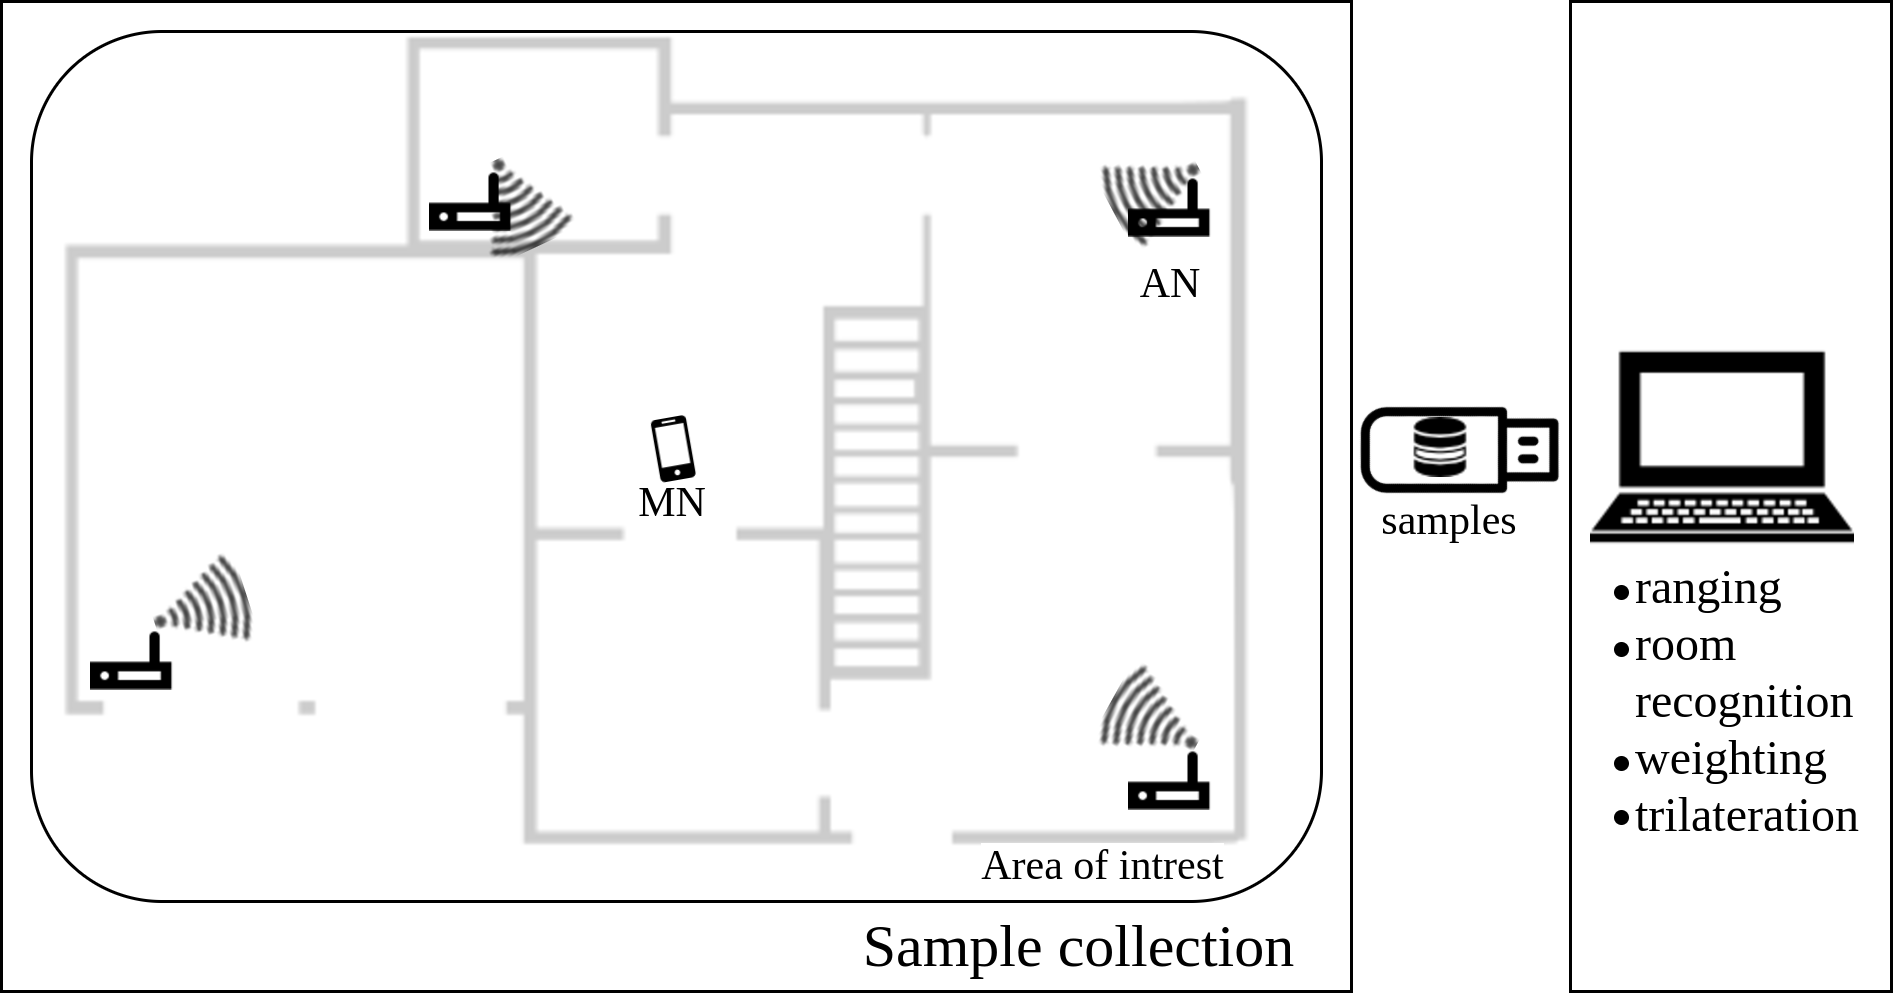
\includegraphics[width=\textwidth]{Figures/SystemImplementationOverview}
\decoRule
\caption[Test bed implementation overview]{Overview of the test bed implementation}
\label{fig:localizationSystemOverview}
\end{figure}

In our test bed implementation the smartphone is only used to collect the samples. On the computer these samples are then used as training and evaluation points for the localization system. This way it is possible to try out and empirically compare different parameters of the system under the exact same conditions.

The set-up of this test bed comprises both hardware and software specific configurations for each component. The remainder of this chapter details these configurations.

\section{Hardware Set-up}

This set-up requires three different kinds of devices. One for the AN, another for the MN and a computer. There are no special requirements for the computer as long as it is able to execute Java code.

For the AN and MN the following hardware was employed:

\paragraph{Anchor Nodes}
The commercial WiFi access points used as anchor nodes are of the model D-Link D-635 and D-2553. They are set-up with a beacon period of 100ms and broadcast on the 2.4 GHz frequency band.

\paragraph{Mobile Node}

The mobile node is an android smartphone of the model \emph{One Plus One}. It has the following specifications:

\begin{itemize}
\item \textbf{OS:} Android 5.1
\item \textbf{Processor:} 2.5GHz Quad-core CPU
\item \textbf{WiFi module:} Qualcomm WCN3680 802.11ac/FM/BT 4.0 Combo Chip 
\item \textbf{Internal sensors:} accelerometer, magnetometer, gyroscope, proximity, ambient light
\item \textbf{Memory:} 3 GB RAM
\end{itemize}

The WiFi module and the magnetometer are used for the sample collection. The magnetometer is reasonably accurate while the off-the-shelf WiFi interface is  prone to interferences.


\section{Software Set-up}

\subsection{Mobile Node}

The mobile node runs an android application which collects RSSI and magnetic field data.

To collect one sample the application takes the average of five RSSI and magnetometer measurements, each spaced 2 seconds apart. The samples are then saved to a \code{.csv} file on the smartphones internal storage so they can later be transferred to the computer.

Each sample consist of:
\begin{itemize}
\item \textbf{A label} aether indicating the room or the exact location where the sample was taken.
\item \textbf{A set of RSSI values}, one for each AN.
\item \textbf{The magnetic field strength} in \(\mu\)-Tesla along the devices x,y and z axis.
\end{itemize}

On android the WiFi module can not be accessed directly. WiFi scans have to be initiated through the \code{AndroidAPI} and it only supports full scans\cite{brouwers2014incremental}. Full scans take longer so it is only possible to take one RSSI measurement every 1.5 seconds.

Due to the low sampling rate it is not practical to apply filters to remove noise from the $RSSI$. It is also not possible to access channel state information which could be used to mitigate some of the multi path effects.

\subsection{Computer}

On the computer a few different programs are used to implement the localization system:
\begin{itemize}
\item \textbf{WEKA 3.6} is used for the room recognition classifier.

\item \textbf{Matlab}'s function fit tool is used to train the ranging model.

\item A \textbf{Spreadsheet} program is used to manually calculate the weighting model.


\item The \textbf{trilateration tool} is responsible for the application of the ranging and weighting models and performs the trilateration. It is a small Java application written for this test bed implementation.

\end{itemize}

The implementation of the room recognition system is split into two phases; The \textbf{offline phase} where the  room recognition, ranging and weighting model are generated. And the \textbf{online phase} where the models are used to predict the location of unknown samples.
 
Figure \ref{fig:offlineImplementation} gives an overview of this process. In the following the two phases are explained in detail.

\begin{figure}[ht]
\centering
\includegraphics[width=\textwidth]{Figures/Offline_Set-Up}
\decoRule
\caption[Test bed offline implementation]{Diagram of the offline implementation}
\label{fig:offlineImplementation}
\end{figure}

\subsubsection{Offline Phase}

\paragraph{Room Recognition Model}
The SVM for the room recognition is trained in WEKA. It generates a multiclass SVM model from the training data set and may use grid search for the parameter selection. The training data set consists of samples containing RSSI \((RSSI_{i})\) and magnetic field \((B_{xyz})\) values labeled with the room number \((R\#)\).

\paragraph{Ranging Model}
For the ranging model the \(\alpha, \beta\) parameters from equation \ref{eqn:non-linear path loss model} need to be determined for each AN. This is done by fitting the equation to the testing data in \emph{Matlab}. The testing data set is a list of RSSI values and the corresponding distance \((D_{i})\) to the AN.

The resulting non-linear regression model is inaccurate with high RSSI values (samples very close to the AN). To account for that the distances for these high values are set by hand.

\paragraph{Weighting Model}

The \emph{Room Weights} are calculated by hand based on equation \ref{eqn: Room Weights} in a spreadsheet program and imported into the trilateration tool.

The \emph{Distance Weights} are calculated by the trilateration tool during run time based on the equation \ref{eqn: distance weights}.

\subsubsection{Online Phase}

The online dataset contains samples with RSSI and magnetic field values.

In a first step WEKA is used to predict the room number. The result is handed to the trilateration tool, which applies the ranging and weighting models to determine the predicted distances \((d_{i})\) and calculate the weights \((w_{i})\). It then solves the trilateration problem (equation \ref{eqn: trilateration as optimization problem}) using the Levenberg–Marquardt optimizer from the \code{Apache Commons Math} library. It outputs the predicted position \((x,y)\) to a \code{.csv} file.

To evaluate the system, the online dataset can also contain the actual position \((X,Y)\) where the sample was collected. In this case the trilateration tool will also output the localization error.
 
%\chapter{Evaluation}
\newcommand{\rd}[1]{\textcolor{red}{#1}}
\newcommand{\gn}[1]{\textcolor{green}{#1}}

\label{Chapter5}

In chapter \ref{Chapter4} the test bed implementation was introduced. In this chapter this test bed is used to evaluate the performance of the system proposed in chapter \ref{Chapter3}.

The evaluated components of the system are the room recognition and the room based weighting method for the trilateration.

Before presenting the evaluation results section \ref{TestBedDeployment} introduces the environment where the test bed was deployed and the data sets used for the evaluation. Sections \ref{EvaluationRoomRecognition} and \ref{EvaluationWeighting} then evaluate the room recognition and weighting method.

\section{Test bed deployment and collected data sets}
\label{TestBedDeployment}

\begin{figure}[ht]
\centering
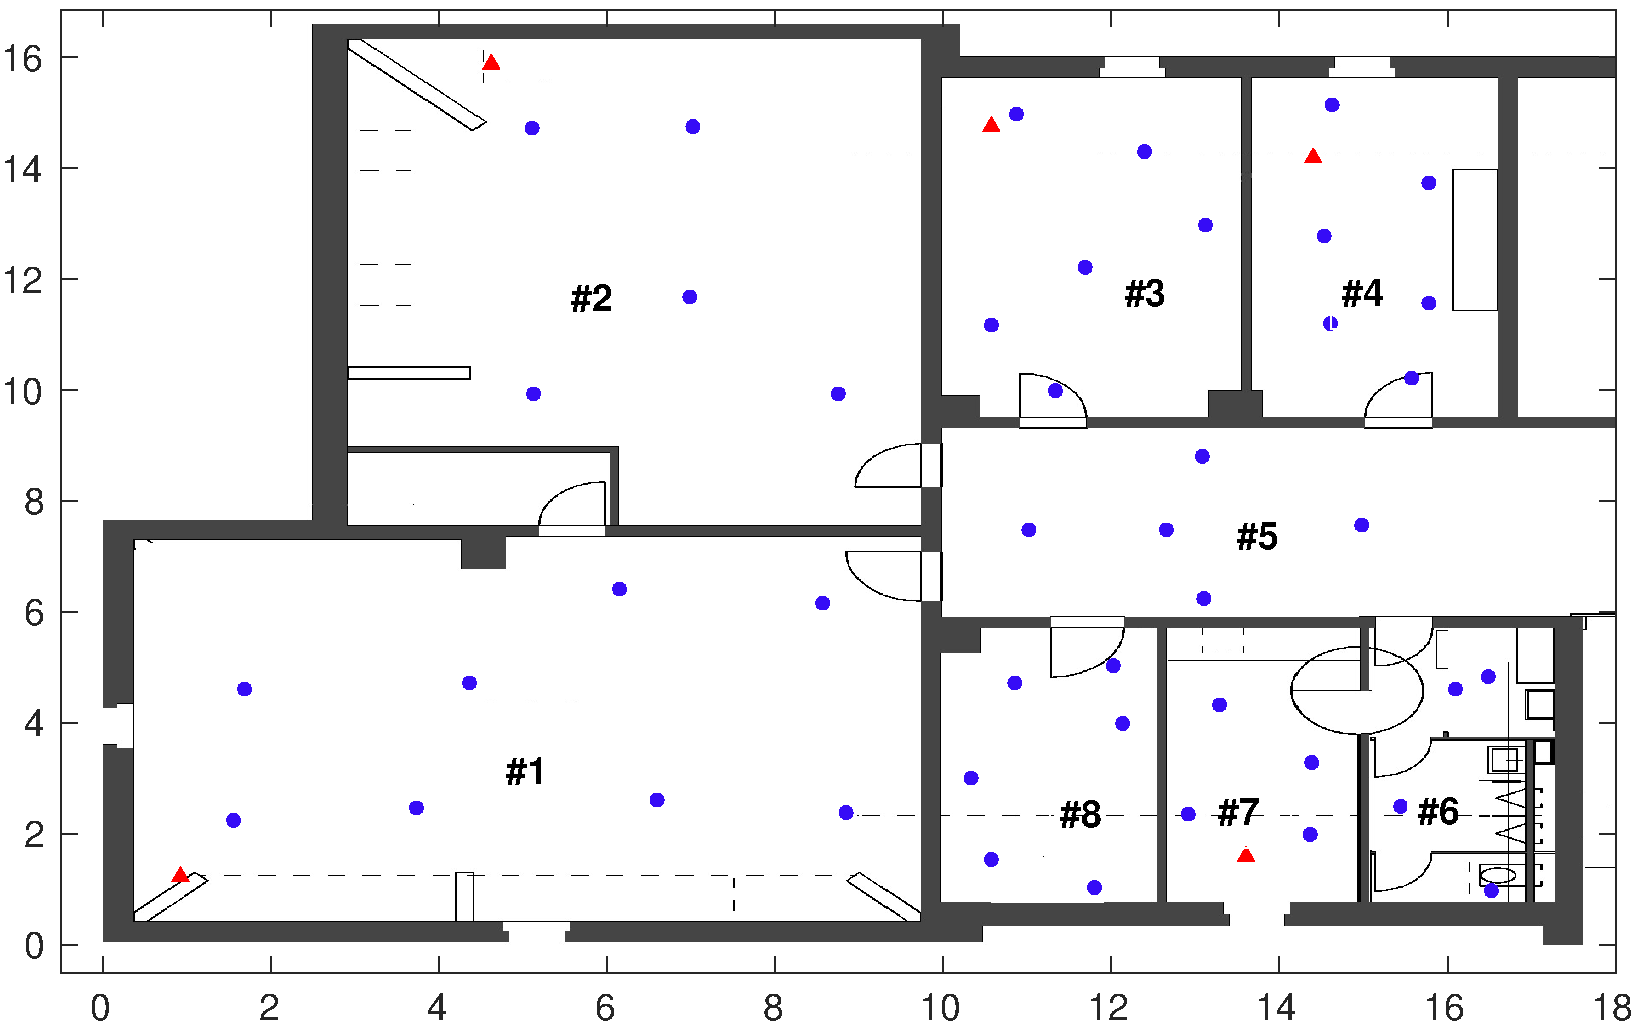
\includegraphics[width=\textwidth]{Figures/FloorPlan_ANs}
\decoRule
\caption[Floor plan]{Floor plan showing the area of interest with the anchor nodes in red, the \emph{XY}-samples in blue and the room numbers in black}
\label{fig:FloorPlanANs}
\end{figure}

The test bed was deployed on the third floor at the Institute of Computer Science (INF) of the University of Bern. The area of interest is 297m\textsuperscript{2} in size, with seven rooms connected by a large corridor. The five anchor nodes were positioned to provide maximum coverage of the area so that the mobile node is able to receive at least four of the signals at all time. The rooms were given numbers from one to eight, the corridor being also treated as a room.

\paragraph{Collected Data Sets} The samples were collected with the smartphone held approximatively one meter above the ground and always pointing in the same cardinal direction. This is important because the magnetic field measurements are influenced by the devices orientation.

The collected samples were grouped into the following data sets:

\begin{itemize}
\item \textbf{Room recognition data} \textbf{only} labeled with the room number
	\begin{itemize}
	\item \textbf{Grid:} 223 samples \textit{(green dots in Figure \ref{fig:DataSets})}

	A set of \textbf{evenly distributed} samples gathered in a grid pattern with approximately 1.2m distance between them.
	\item \textbf{Borders} 373 samples \textit{(red dots)}

	A set of \textbf{unevenly distributed} samples. The sample density is very high at the borders (walls and doors between rooms) with about one sample taken every 0.5m but only a few samples from the center of each room.\\
	\textit{red dots in Figure \ref{fig:DataSets}}
	\end{itemize}
 \item \textbf{XY data} labeled with the exact coordinates \textit{(blue dots)}\\
A set of 44 \textbf{evenly distributed} samples labeled with \((X,Y)\)-coordinates \textbf{and} room number. Figure \ref{fig:FloorPlanANs} shows them as blue dots.
\end{itemize}

Figure \ref{fig:DataSets} visualizes the difference between the data sets. The points are examples and not identical to the actual samples in the data sets.

The room recognition data sets (\emph{Grid}, \emph{Borders}) are used to train the room recognition model. The \emph{XY} data set is mainly used to train the ranging model and evaluate the trilateration accuracy. But we can also use it as an independent test set to compare and evaluate the room recognition models.

\begin{figure}[bh]
\centering
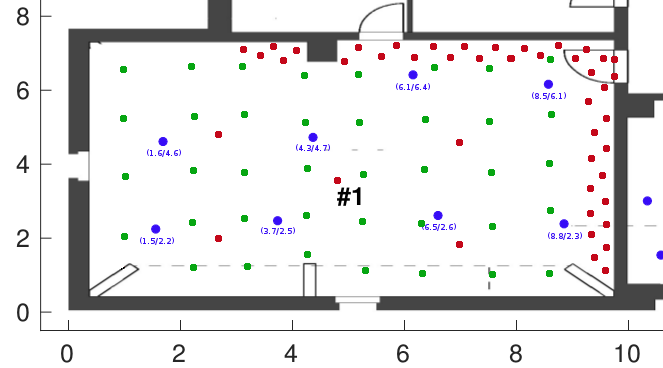
\includegraphics[width=\textwidth]{Figures/DataSets.png}
\decoRule
\caption[Collected Data Sets]{Illustration showing room \#1 and the collected data sets. (blue) \emph{XY} data set with exact coordinates, (green) \emph{Grid} data set, (red)\emph{Borders} data set.}
\label{fig:DataSets}
\end{figure}

\section{Room Recognition}
\label{EvaluationRoomRecognition}

The purpose of this evaluation is to check the hypothesis that the magnetic field data improves room recognition accuracy. Additionally, we want to find out what kind of training data (evenly distributed or more samples at the borders) achieves the best results.

\paragraph{To check if the magnetic field data has a significant impact on the performance of the room recognition} We perform a 10-fold cross validation\cite{crossvalidation} on the evenly distributed \emph{Grid} data set both with and without using magnetic field data. The resulting accuracies are compared. This experiment is repeated with different SVM parameters to see if the parameters have an impact on the result.

\paragraph{To determine the best training data set} Multiple models are generated using the two training data sets (\emph{Grid}, \emph{Borders}) and different SVM parameters and kernels. The models are tested against the evenly distributed \emph{XY} data set and the resulting accuracies are compared.

For the SVM parameters we use WEKA's standard pre-set values as well as optimized parameters selected with cross validation and grid search.

\paragraph{Results: Magnetic field data}

Table \ref{tab:RoomRecognitionMagneticField} shows a large difference between the performance with and without magnetic field data when using cross validation. With WEKA's pre-set SVM parameters (poly-kernel, $c=1,e=1$) the improvement is very large with almost 20\%. When using the optimal parameters (determined by grid search for each case separately) the difference drops to a still significant 10\%. This drop is due to the fact that the pre-set parameters seem to be better suited to the case with magnetic field data. A comparison between the two cases using not optimal parameters is therefore unfair.

Cross validation can sometimes be a little biased. So the impact of magnetic field data was also compared by training with the \emph{Grid} data set and testing against the \emph{XY} data set, mimicking a real-world use case of the room recognition. Surprisingly this only resulted in a 2.3\% improvement.



\begin{table}
\centering
\begin{tabular}{l l l l}
\toprule
\textbf{Evaluation Type}&\textbf{with }\boldmath$B_{xyz}$&\textbf{without }\boldmath$B_{xyz}$&\textbf{Improvement} \\
\midrule
CV (pre-set)&90.1\%&70.4\%&19.7\%\\
CV (optimized)&93.3\%&83.0\%&10.3\%\\
Train: \emph{Grid}, Test: \emph{XY}&84.1\%&81.8\%&2.3\%\\
Train: \emph{Grid}, Test: \emph{XY}&97.3\%&86.8\%&10.5\%\\
\textit{(without room \#3)}&&\\
\bottomrule
\end{tabular}
\caption[Room Recognition - Magnetic Field improvements]{Accuracy of the room recognition with and without magnetic field data.}
\label{tab:RoomRecognitionMagneticField}
\end{table}

The reason for this unexpected result can be found by comparing the impact of the magnetic field data on the  room recognition accuracy for each room. We see in table \ref{tab:RoomRecognitionPerRoom} that the accuracy is improved in every room where it was not already 100\%, except for room \#3 where the accuracy drops to 0\%.

At the time the data sets were collected room \#3 was almost empty while the two adjacent rooms contained server racks and technical equipment (near the walls separating the rooms). We expect that some of this equipment caused a disruption of the magnetic field during the time that the \emph{XY} data set was created and therefore obscured the already weak magnetic signature of room \#3. A similar effect was observed in related work \citep{Li2012feasableMagnetic}.

When room \#3 is excluded from the test set we get the expected 10\% improvement when using magnetic field data.

\begin{table}
\centering
\begin{tabular}{l l l l}
\toprule
\textbf{Room Number}&\textbf{with }\boldmath$B_{xyz}$&\textbf{without }\boldmath$B_{xyz}$&\textbf{Improvement} \\
\midrule
\#1&100.00\%&100.00\%&-\\
\#2&100.00\%&100.00\%&-\\
\#3&0.00\%&50.00\%&-50.00\%\\
\#4&100.00\%&83.30\%&16.70\%\\
\#5&100.00\%&80.00\%&20.00\%\\
\#6&100.00\%&75.00\%&25.00\%\\
\#7&100.00\%&100.00\%&-\\
\#8&83.30\%&66.70\%&16.60\%\\
\bottomrule
\end{tabular}
\caption[Room Recognition - Accuracy per room]{Accuracy of the room recognition for each room (\emph{XY} test set, poly-kernel, optimized parameters)}
\label{tab:RoomRecognitionPerRoom}
\end{table}

\paragraph{Results: Data sets and SVM parameters}

Table \ref{tab:SVMconfigurationPresets} shows the accuracy for the two training data sets and two different kernel functions using WEKA's pre-set parameters. The polynomial kernel performs very well while with the RBF kernel the accuracy is below 20\% for all training data sets. The RBF kernel, with these parameters, does not seem to be a good fit for this kind of data.

With the polynomial kernel the unequally distributed \emph{Borders} data performs better. But it is only 2.3\% better than \emph{Grid}, which has 40\% fewer samples. This difference does not seem significant and is most likely due to the higher numbers of samples.

Table \ref{tab:SVMconfigurationPoly} shows the accuracy with optimal parameters for each training set and kernel. The parameters were selected with a grid search.

For both training data sets the accuracy could be slightly increased by the parameter selection, but the relative accuracy is still the same; \emph{Borders} has the highest performance with \emph{Grid} only being marginally worse.

With the optimized parameters both kernels have a similar performance, although the RBF kernels $c$ values are generally higher. A high $c$ value means that the RBF kernel's decision surface needs to be more complex and have a smaller margin to achieve the same accuracy as the polynomial kernel. In general a less complex decision surface with a higher margin is preferred. We therefore infer that the polynomial kernel is better suited for this problem.

Finally, to see if it is possible to train a room recognition system with a minimal number of samples the system was trained with the \emph{XY} data set and tested against the \emph{Grid}. This resulted in an accuracy of 81.2\%. This is still very high considering only 44 training samples were used.



\begin{table}

\centering
\begin{tabular}{l l l}
\toprule
\textbf{Training Data}&\textbf{Polynomial}&\textbf{RBF}\\
\textbf{(\#Samples)}&$c=1,e=1$&$c=1,g=0.01$\\
\midrule
Grid (223)&81.8\%&18.2\%\\
Borders (373)&84.1\%&11.4\%\\
\bottomrule
\end{tabular}
\caption[Room recognition - SVM pre-sets]{Accuracy of the room recognition with different training data sets using the polynomial and RBF kernel pre-sets}
\label{tab:SVMconfigurationPresets}
\end{table}

\begin{table}
\centering
\begin{tabular}{l l l l l l l}
\toprule
\textbf{Training Data}&\multicolumn{3}{c}{\textbf{Polynomial}}&\multicolumn{3}{c}{\textbf{RBF}}\\
\textbf{(\#Samples)}&\textbf{accy}&$c$&$e$&\textbf{accy}&$c$&$g$\\
\midrule
Grid (223)&84.1\%&10&1&84.1\%&100&0.01\\
Borders (373)&88.6\%&100&1&86.4\%&1000&0.01\\
\bottomrule
\end{tabular}
\caption[Room Recognition - optimized parameters]{Accuracy of the room recognition with different training data sets using the optimal parameters}
\label{tab:SVMconfigurationPoly}
\end{table}

\newpage

\section{Weighting}
\label{EvaluationWeighting}

Section \ref{EvaluationRoomRecognition} has shown that the proposed room recognition can achieve high accuracy even with a small training data set. Potentially it could be trained with the same points used to train the ranging model, eliminating the need to collect additional samples. It is now possible to evaluate the proposed weighting method and see if the information from the room recognition can be used to improve the range based localization accuracy.

In Chapter \ref{Chapter3} a new weighting method was proposed; the \emph{Room Weights} (equation \ref{eqn: Room Weights}). The goal of this evaluation is to evaluate if the \emph{Room Weights} improve the accuracy of the trilateration and if this is true whether the accuracy can be further improved by combining the \emph{Room Weights} with the existing method of the \emph{Distance Weights}.

In a first step the new weighing method is applied with the assumption of 100\% room recognition and compared to \emph{ordinary least squares} (trilateration with no weights). This gives us a best-case value for the improvements with the new weighting method.

In a second step the weighting method is applied to a real word scenario using a room recognition system trained with the \emph{Grid} data set (accuracy of 84\%). The results are compared to the 100\% case to see how sensitive the weighing method is to errors in the room recognition.

Finally, the performance of the proposed weighting method under real world conditions is compared to the \emph{Distance Weights} to see if it performs better than other simpler weighting methods.

The \emph{ranging model} and \emph{room weights} are trained with the entire \emph{XY} data set and imported into the trilateration tool. For evaluation the same data-set is used.

\paragraph{Results}
In addition to the mean, standard deviation and maximum error, the results are presented as the cumulative distribution function of the localization error. This allows for a more accurate representation of the performance than just using statistical values.

\begin{table}[ht]
\centering
\begin{tabular}{l l l l l}
\toprule
\textbf{Weighting Method}&\textbf{Mean}&\textbf{STD}&\textbf{Max}&\textbf{Improv}\\
&&\textbf{}&\textbf{Error}&\textbf{over OLS}\\
\midrule
OLS&2.74m&1.57m&8.25m&\\
Room Weights (100\%)&2.35m&1.22m&4.89m&14.2\%\\
Room+Distance Weights (100\%)&2.29m&1.16m&4.65m&16.4\%\\
Room+Distance Weights (84.1\%)&2.40m&1.25m&5.69m&12.4\%\\
Distance Weights&2.42m&1.19m&5.37m&11.3\%\\
\bottomrule
\end{tabular}
\caption[Weighting - statistical values]{Comparison of the statistical values for the different weighting methods}
\label{tab:WeightingStatisticalValues}
\end{table}

\begin{figure}[p]
\centering
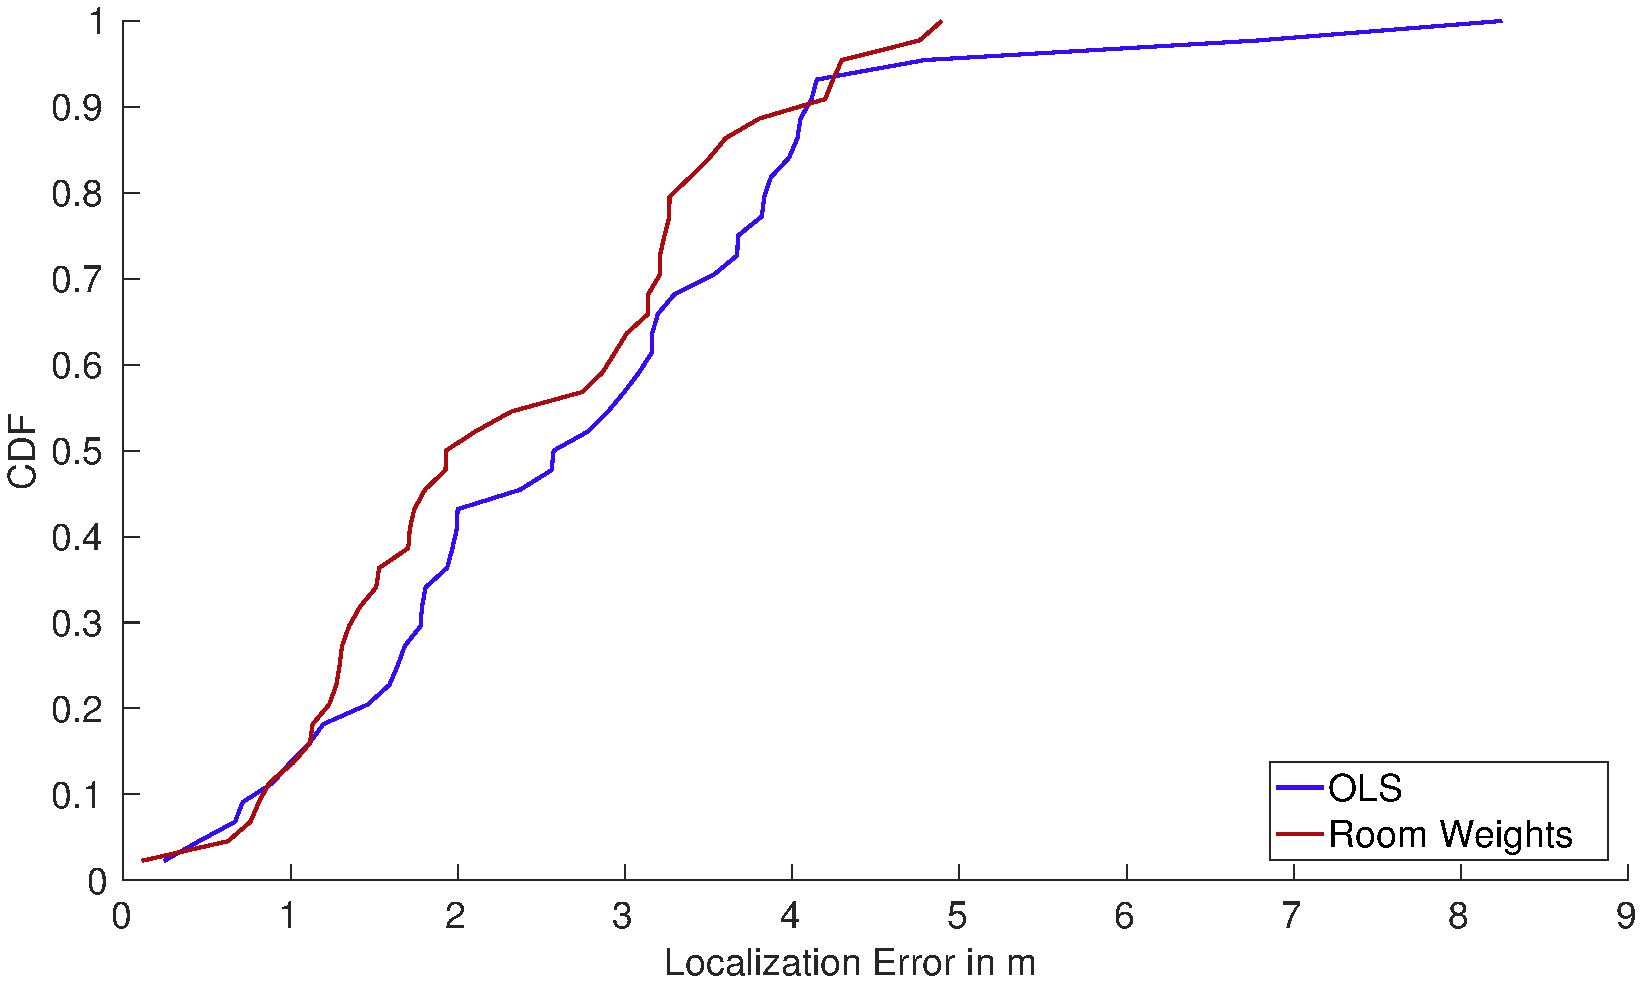
\includegraphics[width=\textwidth]{Figures/WeightingCDF_RW}
\decoRule
\caption[CDF Room Weights method (best-case)]{The Localization error with the \emph{Room Weights}.}
\label{fig:WeightingCDFRoom}
\end{figure}

\begin{figure}[p]
\centering
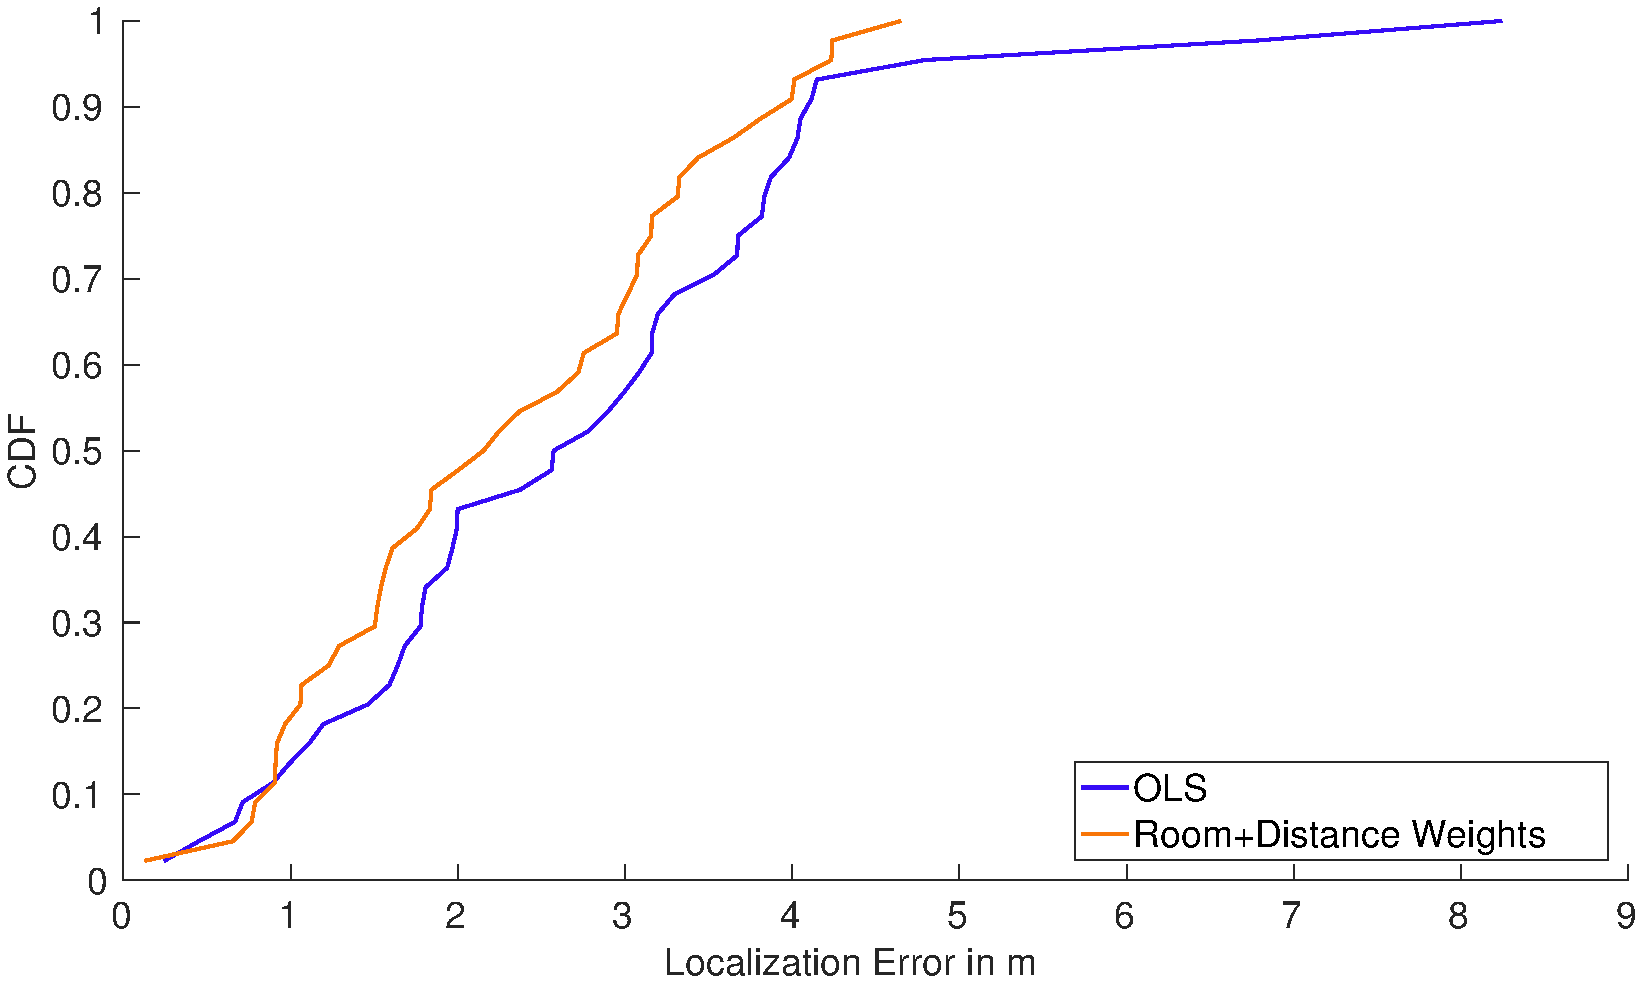
\includegraphics[width=\textwidth]{Figures/WeightingCDF_RDW}
\decoRule
\caption[CDF Room+Distance Weights method (best-case)]{The Localization error with the \emph{combined room and distance weights}.}
\label{fig:WeightingCDFRoomDistance}
\end{figure}

The results with 100\% room recognition show an improvement of the \emph{Room Weights} over \emph{OLS}. The mean error is 14.2\% ($\approx$0.4m) lower, the standard deviation smaller and the maximum error was reduced by $\approx$3.4m. But when looking at the CDF plot (Figure: \ref{fig:WeightingCDFRoom}) the improvement, although visible, does not seem very dramatic and is mainly due to the large reduction in the maximum error.

The results also show that combining the \emph{Room} and \emph{Distance Weights} does indeed yield a further small improvement. While the mean error is only marginally increased, it lowers the maximum error even further and smooths out the CDF curve (Figure: \ref{fig:WeightingCDFRoomDistance}).

The comparison between the performance of the weighting in a best-case scenario and real world case, shows that there is indeed an error introduced by the room recognition. But the CDF (Figure: \ref{fig:WeightingCDFrealRoom}) shows that this error is overall very small and mainly due to a few samples with a large error, which increase the maximum error.

However, when taking into account this error, the real world performance of the proposed weighting method is almost the same as the existing simpler \emph{Distance Weights}. This is apparent in Figure \ref{fig:WeightingCDFrealDistance}. The mean error is only a few centimeters lower (0.07m) and the maximum error even higher than with the \emph{Distance Weights}.

\begin{figure}[bh]
\centering
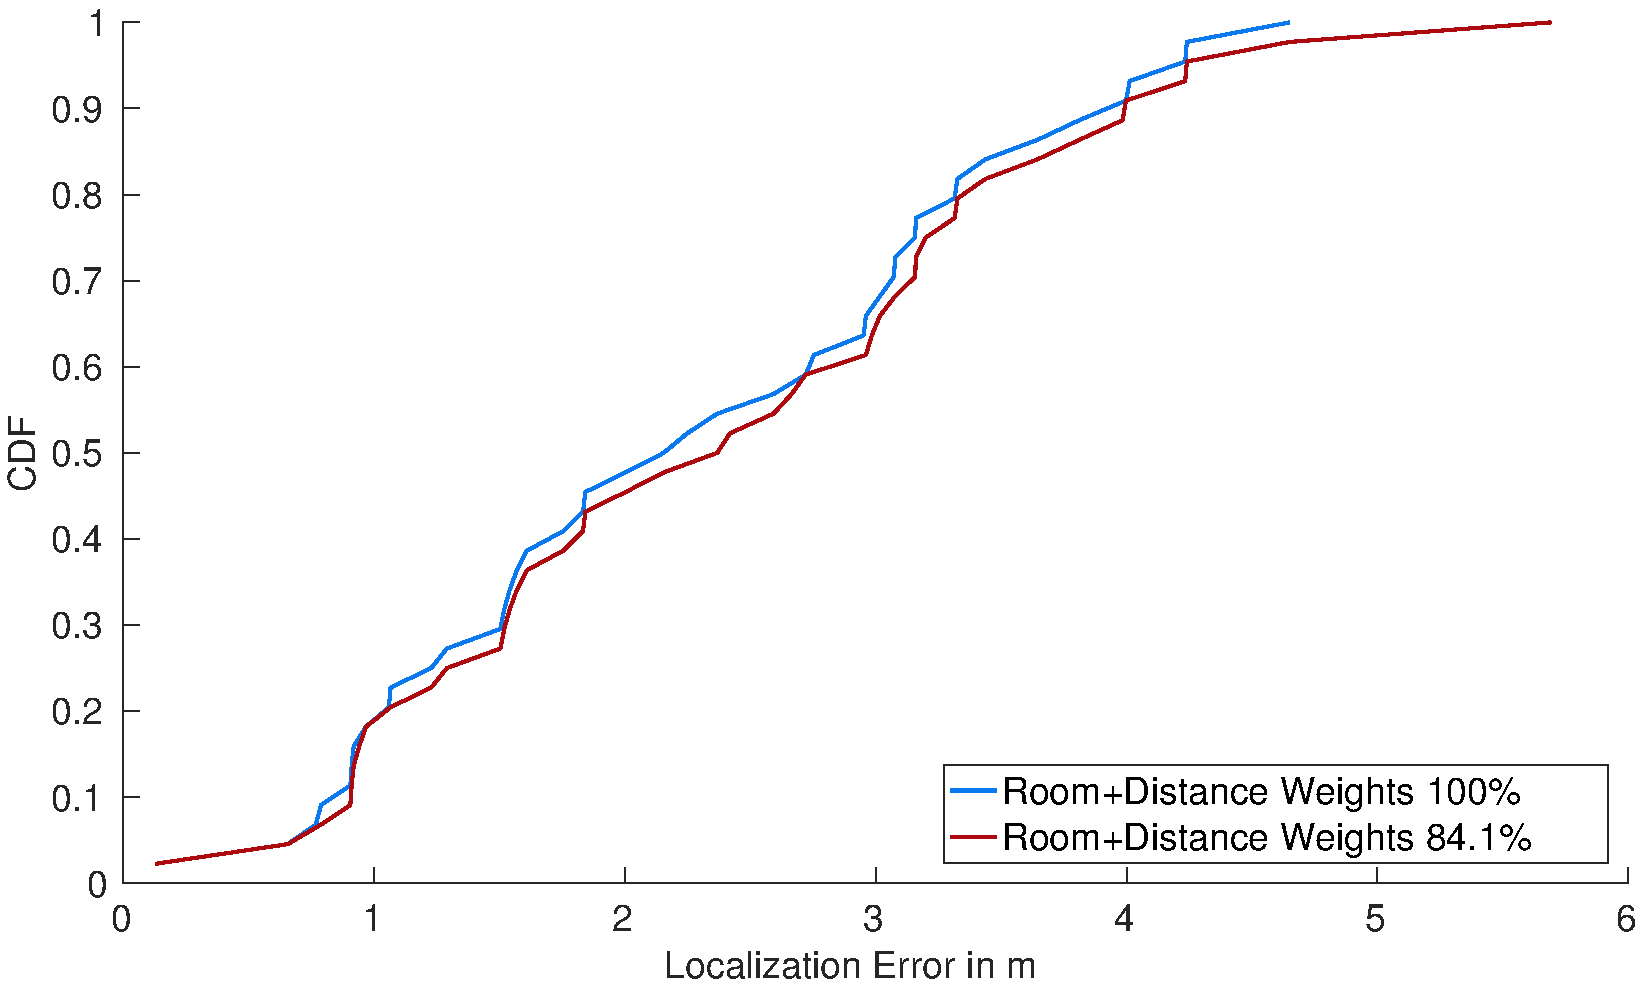
\includegraphics[width=\textwidth]{Figures/WeightingCDF_realRW}
\decoRule
\caption[CDF Room+Distance Weights - best-case/real world comparison]{Localization error with \emph{combined room and distance weights} in a best-case and real world scenario}
\label{fig:WeightingCDFrealRoom}
\end{figure}

\begin{figure}
\centering
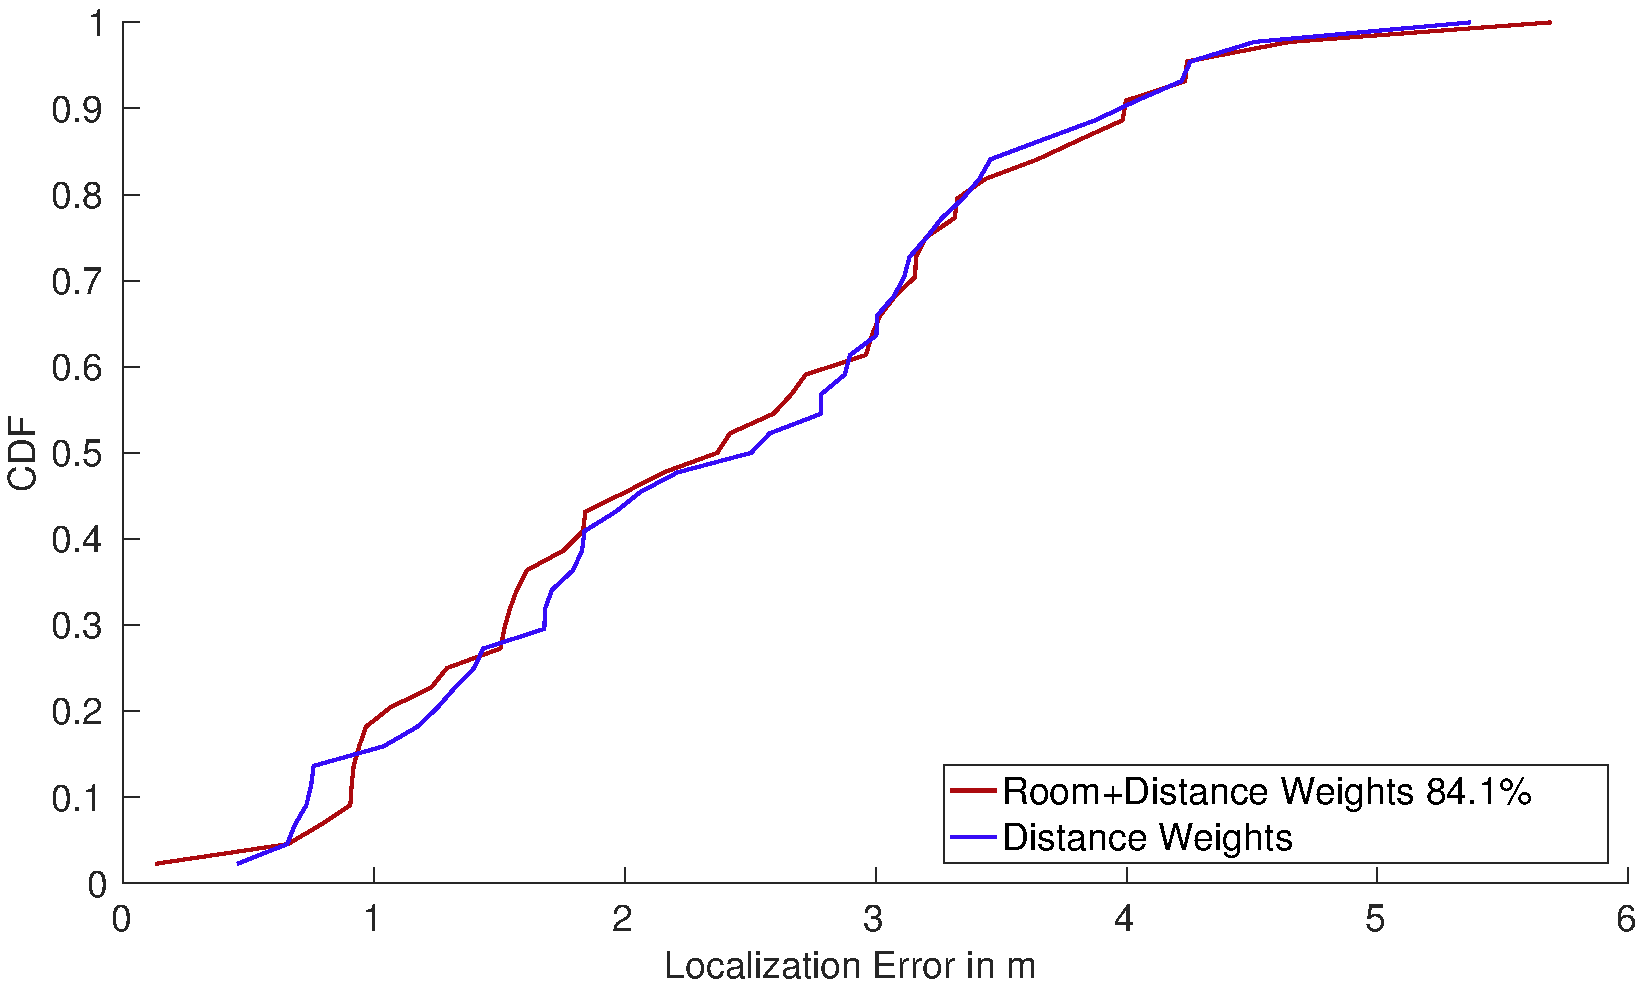
\includegraphics[width=\textwidth]{Figures/WeightingCDF_realDistance}
\decoRule
\caption[CDF Room+Distance Weights - comparison against Distance Weights]{Localization error for the \emph{combined room and distance weights} and \emph{Distance Weights}}
\label{fig:WeightingCDFrealDistance}
\end{figure}
 

%----------------------------------------------------------------------------------------
%	THESIS CONTENT - APPENDICES
%----------------------------------------------------------------------------------------

\appendix % Cue to tell LaTeX that the following "chapters" are Appendices

% Include the appendices of the thesis as separate files from the Appendices folder
% Uncomment the lines as you write the Appendices

% Appendix A

\chapter{Appendix Title Here} % Main appendix title

\label{AppendixA} % For referencing this appendix elsewhere, use \ref{AppendixA}

Write your Appendix content here.
%\include{Appendices/AppendixB}
%\include{Appendices/AppendixC}

%----------------------------------------------------------------------------------------
%	BIBLIOGRAPHY
%----------------------------------------------------------------------------------------

\printbibliography[heading=bibintoc]

%----------------------------------------------------------------------------------------

\end{document}  
